\section{Introduction}

Depression has been a major health challenge to the world, with over 280 million people affected, according to WHO\footnote{\url{https://www.who.int/news-room/fact-sheets/detail/depression}}. Moreover, the COVID-19 pandemic has further deteriorated the situation. 
%COVID patients are more likely to suffer from depression due to poor health condition as well as perceived stigmatization.
% \cite{mazza2020anxiety}  % can't add due to the 1 page limitation of references
Since people are more 
willing to express their feelings on online social media during this 
special period\footnote{\url{https://www.statista.com/statistics/1106498/home-media-consumption-coronavirus-worldwide-by-country/}}, 
depression detection from online posts can be a promising approach 
to combat the challenge.
The conventional setting of depression detection from online posts is to predict whether a user suffers from depression from the whole posting history \cite{gui2019cooperative,zogan2021depressionnet}. However, for social networks which update quickly, 
another setting, \textit{early risk detection} (ERD)~\cite{losada2017erisk}, 
may have more potential to detect and offer timely help to risky users. 
An ERD model should access user post one by one sequentially, 
dynamically update the estimated risk, and make immediate alert once 
it is confident enough about its prediction. This setting is less explored due to 
its unique challenges: 

First, the ability of classification on streaming data is a requirement of ERD models. This means that the method is better to be an online, incremental algorithm that can update the prediction every time a user sends a post, rather than an offline batch algorithm that only runs once after a long interval. Since traditional ML models do not 
come with such ability inherently, a typical solution is to naively process 
the whole posting history for each update~\cite{trotzek2018utilizing}. 
This method can hardly be efficient enough in practice. 
For instance, many systems in an ERD competition, eRisk2019, spent several 
days for computation~\cite{losada2019overview}. 
% Another approach is to make predictions only from the latest post instead of the posting list \cite{bucur2021early}. Nonetheless, such methods may lose the potential of leveraging the useful history information for better accuracy.

Moreover, an ERD model should make tradeoff between its timeliness and accuracy. 
To make an early prediction, the model usually predicts a depression probability 
after each update, and makes an alert if the probability exceeds certain threshold, and we can tune the threshold to control the latency of prediction \cite{trotzek2018utilizing}. Leveraging more posts can certainly facilitate higher accuracy, while it also means that the model makes late predictions, and it fails to make alert before the patient's condition deteriorates. To realize the pareto improvement of both objectives, 
we should also seek improved model structure. 
Although large pretrained Language models (LMs) like BERT~\cite{devlin2018bert} 
has achieved great success in many classification tasks, 
they are seldom applied to ERD, as the long posting history make 
the memory cost and latency prohibitive. 
% Therefore, traditional ML models or relatively small CNN/RNN-based models still dominate the task. 

Due to the sensitiveness of depression detection, model explainability is also 
a vital property. Without proper explanations, it can be hard for users to trust such novel tools and accept these alerts. Since 
deep learning models are mostly black-boxes, one cannot ascertain whether their
predictions are achieved due to robust features, or some spurious clues~\cite{ribeiro2020beyond}. Traditional ML models can provide global explanations of the prediction (i.e., feature importance) based on features like word counts. However, it is much
more preferable if we can make personalized, symptom-based explanations~\cite{mowery2017understanding} like psychiatrists to endow higher level of trustworthiness. 

\begin{figure}[t]
    \centering
    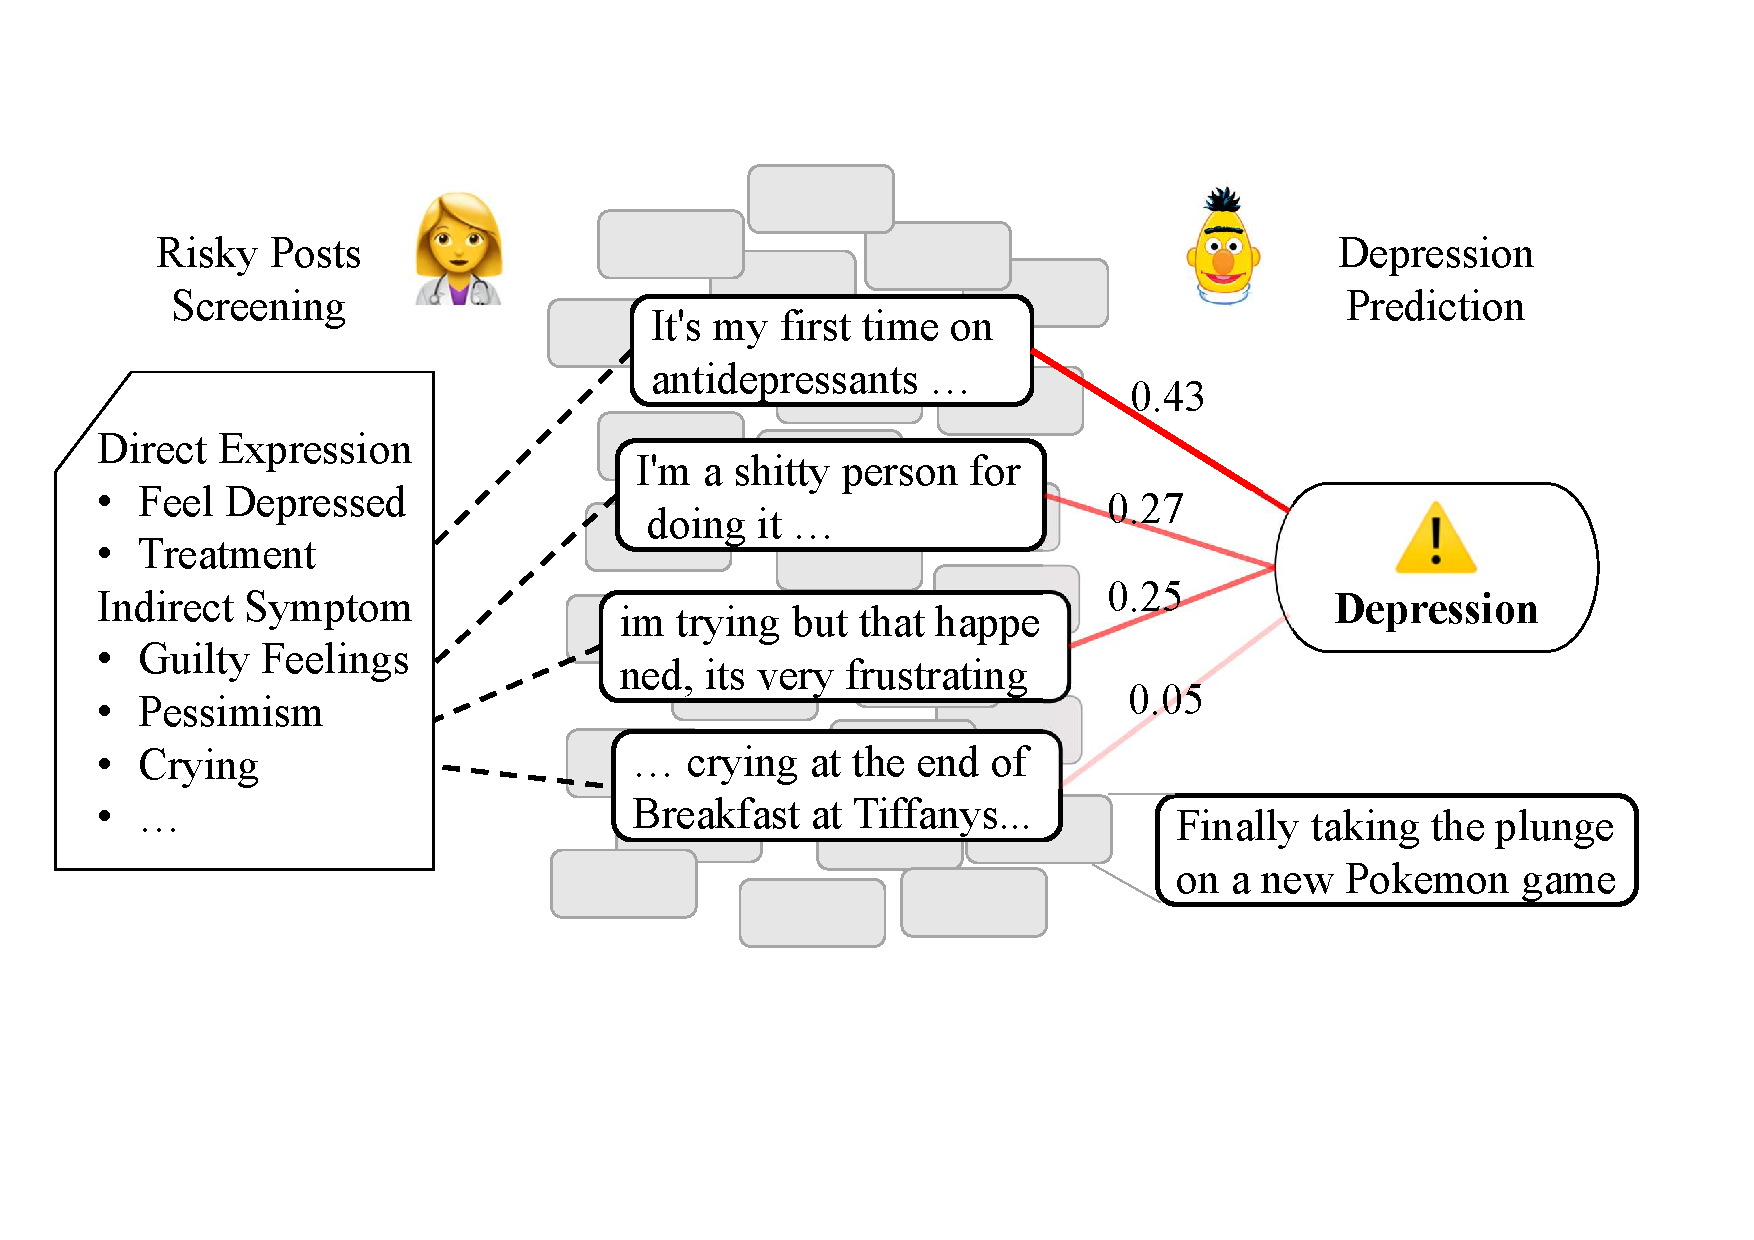
\includegraphics[width=\columnwidth]{figures/overview1.pdf}
    \caption{Overview of the system. Depression templates derived from established depression scales are used to screen risky posts, and filter out safer ones (boxes in grey). A hierarchical attentional network further attends to truly important contents (darkness of red lines indicates attention strength) and makes final prediction. }
    \label{fig:overview}
\end{figure}

Inspired by the psychiatry practice of using clinical scales to screen depression patients, we propose to use depression templates derived from established depression scale \cite{beck1996beck} to screen risky posts. These templates include direct expressions of depressive moods and depression treatments, as well as theory-grounding indirect symptoms like guilty feelings, pessimism and loss of appetite, etc. Only posts highly relevant to these templates will be selected out of the whole posting history, which can greatly reduce the input size, so as to eliminate distractors and improve processing efficiency. A hierarchical network incorporating attention mechanism \cite{yang2016hierarchical} and BERT \cite{devlin2018bert} further aggregates the selected posts of a user, and assigns higher weights to truly important contents for accurate and explainable predictions. The overview of our approach is illustrated in Figure \ref{fig:overview}. To enable ERD, we also propose an online algorithm based on a risky posts queue evolving with the streaming posts. Experimental results show that the proposed method can achieve SOTA performance in both conventional and ERD settings, and can be even a more efficient ERD solution than simple Logistic Regression models.

Our key contributions are as follows: 
1) We propose psychiatry-guided risky post screening to select salient contents for processing, which reduces the input size so as to allow the utilization of large models, and can provide symptom-based interpretations.
2) We leverage hierarchical attentional network with BERT (HAN-BERT) to enhance the model accuracy and explainability.
3) We propose an online algorithm based on an evolving queue of risky posts to tackle ERD, achieving simultaneous improvement in timeliness and accuracy over representative baselines. 
